{\normalsize Baseado nas listas de exercícios}

\section{Redes Cristalinas}


\begin{itemize}
	\setlength{\parskip}{0pt}
	\setlength{\itemsep}{0pt plus 1pt}
	
	\item NC: Número de Coordenação
	\item FE: Fator de empacotamento
\end{itemize}


Cubo simples - CS




\begin{itemize}
	\item NC: 6;
	\item FE: $\frac{4}{3} \cdot \frac{\pi \cdot r^{3}}{a^{3}} = 0,52$;
	\item Rel: $a = 2R$;	
\end{itemize}


Cúbico de Corpo Centrado - CCC

\begin{itemize}
	\item NC: 8
	\item FE: $2 \cdot \frac{4}{3} \cdot \frac{\pi \cdot r^{3}}{a^{3}} = 0,68$
	\item Rel: $a = \frac{4R}{\sqrt{3}}$
\end{itemize}


Cúbico de Faces Centradas - CFC

\begin{itemize}
	\setlength{\parskip}{0pt}
	\setlength{\itemsep}{0pt plus 1pt}
	
	\item NC: 12
	\item FE: $4 \cdot \frac{4}{3} \cdot \frac{\pi \cdot r^{3}}{a^{3}}$ 0,74
	\item Rel: a = $\frac{4 \cdot R}{\sqrt{2}}$
\end{itemize}

Hexagonal

\begin{itemize}
	
	\setlength{\parskip}{0pt}
	\setlength{\itemsep}{0pt plus 1pt}
	
	\item NC: 12
	\item FE: 0,73 (=CFC)
	\item Rel: a = 2R
\end{itemize}


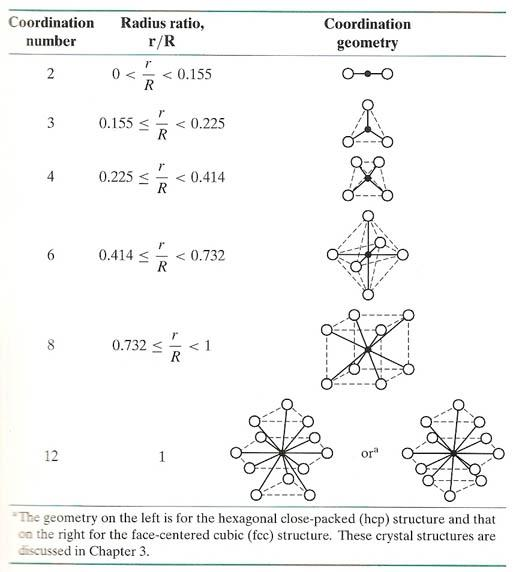
\includegraphics[scale=0.3,trim={0 0 0 0}]{figures/RELraio}


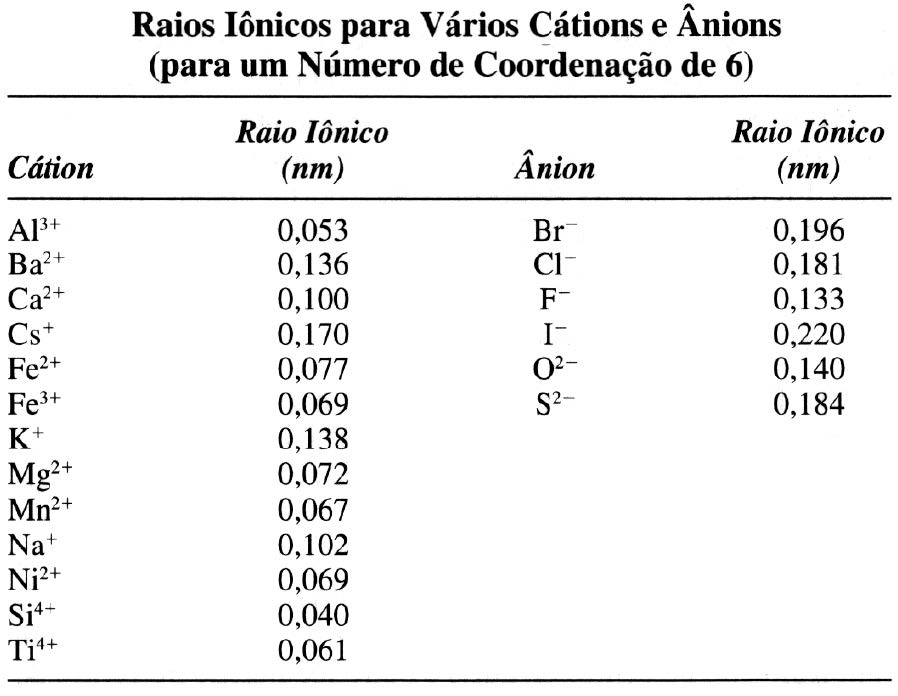
\includegraphics[scale=0.2,trim={0 0 0 0}]{figures/raio}

\section{Variação Vol pela Mudança de Estrutura Cristalina}

Ao avaliar redução de volume resultada pela mudança de estrutura cristalina de um material que durante o seu aquecimento/resfriamento devemos levar em consideração o número de átomos que cada uma das estruturas comporta. Outro ponto importante é levar em consideração que o número de átomos é constante e portanto haverá variação na número de células unitárias formadas.


 \section{Estrutura dos materiais Cerâmicos}

O posicionamento das partículas nos materiais cerâmicos depende da relação entre os raios(cátion/ânion) e das cargas envolvidas. Nos vazios (sítios ou interstícios) da rede cristalina se posicionam partículas diferentes das que existem na rede cristalina principal. Em redes compactas há espaços intersticiais, onde as partículas ficam equidistantes do centro do espaço vazio.


\textbf{Posições octaédricas na rede cfc:}

\begin{itemize}
	
	\setlength{\parskip}{0pt}
	\setlength{\itemsep}{0pt plus 1pt}
	
	\item NC: 6
	\item Local:arestas (3 sítios) + centro da célula unitária
	\item Total: 4 partículas (1 por partículas da célula unitária)
\end{itemize}

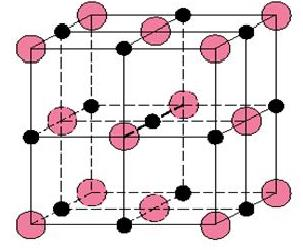
\includegraphics[scale=0.5,trim={0 0 0 0}]{figures/occfc}


\textbf{ Posições tetraédricas na rede cfc:}

\begin{itemize}
	
	\setlength{\parskip}{0pt}
	\setlength{\itemsep}{0pt plus 1pt}
	
	\item NC: 4
	\item Local:posições do tipo ($\frac{1}{4}$, $\frac{1}{4}$, $\frac{1}{4}$)
	\item Total: 8 partículas (2 por partículas	da célula unitária)
\end{itemize}

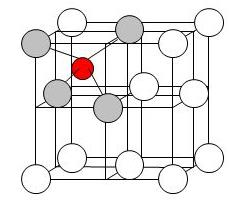
\includegraphics[scale=0.5,trim={0 0 0 0}]{figures/tetcfc}



\section{Contorno de grãos:}

\begin{itemize}
	\item Formada entre cristais (contornos de grãos) ou nas superfícies externas.
	\item No contorno dos grãos, os átomos não estão à mesma distância uns dos outros. Há tensões de tração e compressão.
	\item Influenciam nas propriedades físicas (ex: resistência mecânica) e químicas.
	\item Ajuste do tamanho dos grãos $\rightarrow$ uma das formas de controle das propriedades de um metal.
	\begin{itemize}
		\item Ex: Reduzindo o tamanho dos grãos, há aumento do área de contorno de grão, diminuindo a distância percorrida pelas discordâncias aumento da resistência mecânica do material.
	\end{itemize}
\end{itemize}


\section{Tipos de soluções de materiais metálicos}

\begin{itemize}
	\item Soluções sólidas:
	\begin{itemize}
		\item intersticial
		\item Substitucional:
		\begin{itemize}
			\item Ordenada
			\item Ao acaso
		\end{itemize}
	\end{itemize}
\end{itemize}

\section{Regras de Hume-Rothery para solubilidade}

\begin{itemize}
	\item Variação \% causada pela diferença entre raios < 15\% (evitar distorções na rede): raio soluto = raio solvente/
	\item Mesma estrutura cristalina;
	\item Eletronegatividades semelhantes
	\item Mesma valência.
\end{itemize}



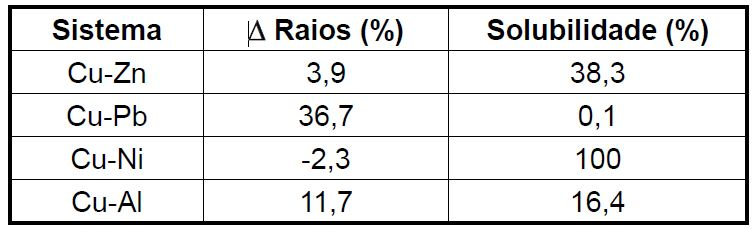
\includegraphics[scale=0.27,trim={0 0 0 0}]{figures/hume}

\section{Definições}

Numero de Coordenação: número de partículas que envolvem uma partícula central.

Fator de empacotamento: volume de átomos numa célula unitária / volume da célula unitária.


\section{Direções Cristalográficas}

A crystallographic direction is defined as a line between two points, or a vector. The following steps are used to determine the three directional indices:

1. A vector of convenient length is positioned such that it passes through the
origin of the coordinate system. Any vector may be translated throughout the
crystal lattice without alteration, if parallelism is maintained.

2. The length of the vector projection on each of the three axes is determined;
these are measured in terms of the unit cell dimensions a, b, and c.

3. These three numbers are multiplied or divided by a common factor to reduce
them to the smallest integer values.

4. The three indices, not separated by commas, are enclosed in square brackets,
thus: [uvw]. The u, v, and w integers correspond to the reduced projections
along the x, y, and z axes, respectively.

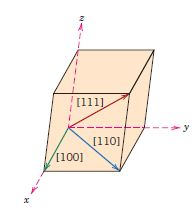
\includegraphics[scale=0.27,trim={0 0 0 0}]{figures/direcoesCrist}

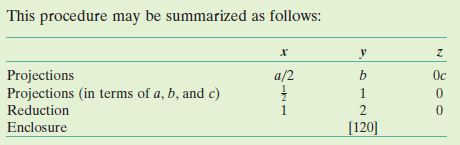
\includegraphics[scale=0.27,trim={0 0 0 0}]{figures/direSum}


\section{Planos Cristalográficos}


1. If the plane passes through the selected origin, either another parallel plane
must be constructed within the unit cell by an appropriate translation, or a
new origin must be established at the corner of another unit cell.

2. At this point the crystallographic plane either intersects or parallels each of
the three axes; the length of the planar intercept for each axis is determined
in terms of the lattice parameters a, b, and c.

3. The reciprocals of these numbers are taken. A plane that parallels an axis
may be considered to have an infinite intercept, and, therefore, a zero index.

4. If necessary, these three numbers are changed to the set of smallest integers
by multiplication or division by a common factor.3

5. Finally, the integer indices, not separated by commas, are enclosed within
parentheses, thus: (hkl).


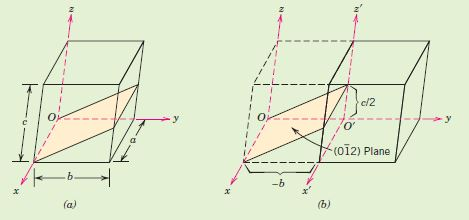
\includegraphics[scale=0.27,trim={0 0 0 0}]{figures/planSum1}

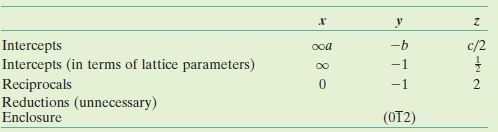
\includegraphics[scale=0.27,trim={0 0 0 0}]{figures/planSum2}


\section{Densidade Teórica}

\begin{equation}\label{key}
\rho=\frac{n A}{V_{c} N_{\mathrm{A}}}
\end{equation}

\begin{itemize}
	\item n = number of atoms associated with each unit cell
	\item A = atomic weight
	\item $V_{C}$ = volume of the unit cell
	\item $N_{A}$ = Avogadro’s number $16.022 \cdot 10^{23} \frac{atoms}{mol^{2}}$
\end{itemize}


\section{Densidade Linear}

\begin{equation}\label{key}
LD = \frac{número de átomos centrados na direção do vetor}{tamanho do vetor direção}
\end{equation}


\section{Densidade Planar}

\begin{equation}\label{key}
PD = \dfrac{número de átomos centrados no plano}{área do plano}
\end{equation}


\subsubsection{Fluxo de Difusão}

A velocidade com que ocorre a difusão é avaliada em termos de FLUXO DE DIFUSÃO que corresponde a massa (ou número de átomos) que se difunde por unidade de tempo através de uma área perpendicular à direção do movimento da massa que está se difundindo.

\begin{equation}\label{key}
J = \frac{M}{(A \cdot t)}
\end{equation}

onde: 

\begin{itemize}
	\item J = fluxo de difusão. $[\frac{Kg}{m^{2} \cdot s}]$ ou $[\frac{át}{m^{2} \cdot s}]$
	\item M = massa transportada (ou quantidade de átomos)
	\item A = área da seção transversal
	\item t = tempo
\end{itemize}


\begin{itemize}
	\item Difusão em estado estacionário
	\item Difusão em estado não estacionário (condições transientes)
\end{itemize}

DIFUSÃO EM ESTADO ESTACIONÁRIO

Condições:

\begin{itemize}
	\item J não varia com o tempo.
	\item J não varia com a posição.
\end{itemize}

PRIMEIRA LEI DE FICK: relaciona o fluxo com o gradiente de concentração

\begin{equation}\label{key}
J = D \cdot \frac{\Delta c}{\Delta x}
\end{equation}

DIFUSÃO EM ESTADO NÃO- ESTACIONÁRIO

Segunda lei de Fick:

\begin{equation}\label{key}
\frac{\partial C}{\partial t}=D \frac{\partial^{2} C}{\partial x^{2}}
\end{equation}

\begin{equation}\label{key}
\frac{C_{\mathrm{X}}-\mathrm{C}_{0}}{\mathrm{C}_{\mathrm{S}}-\mathrm{C}_{0}}=1-\operatorname{erf}\left(\frac{\mathrm{x}}{2 \sqrt{\mathrm{D} \mathrm{t}}}\right), \quad \text { onde } \mathrm{C}_{\mathrm{X}}=\mathrm{C}=\mathrm{f}(\mathrm{x}, \mathrm{t})
\end{equation}

Onde:

\begin{itemize}
	\item x = condição á superfície
	\item $C_{x}$ = Concentração à profundidade x, após tempo t
	\item $C_{0}$ = Concentração inicial da espécie
	\item $C_{s}$ = Concentração na superfície
\end{itemize}


\begin{equation}\label{key}
\operatorname{erf}(z)=\frac{2}{\sqrt{\pi}} \int_{0}^{Z} e^{-y^{2}} d y
\end{equation}


CALCULO DO COEFICIENTE DE DIFUSÃO

\begin{equation}\label{key}
D=D_{0} e^{\left( \frac{-Q_{d}}{R T}  \right)}
\end{equation}

Onde:


\begin{itemize}
	\item $D_{0}$ constante independente da T, em $\frac{m^{2}}{s}$ valores tabelados.
	\item $Q_{d}$ energia de ativação para a difusão $[\frac{J}{mol}]$.
\end{itemize}



